\chapter{さまざまな運動}

注: この章を理解するには, 数学リメディアル教材で三角関数を理解していることが必要である。\mv

\section{単振動}\index{たんしんどう@単振動}
\begin{figure}[h]
    \centering
    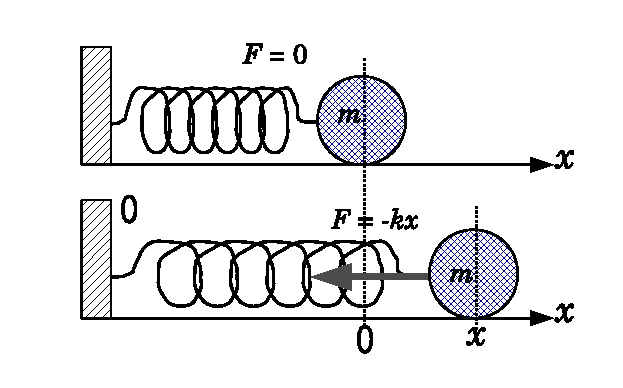
\includegraphics[width=7cm]{spring_vib.eps}
    \caption{バネにつけられて振動する物体}\label{fig:spring_vib}
\end{figure}

図\ref{fig:spring_vib}のように, 壁に一端が固定されたバネの, もう一端に質量$m$の物体がとりつけられた
系を考えよう。物体と床面の間に摩擦は無いものとする。バネ定数を$k$とし, バネ自体の質量は無視する。
バネはこの図の左右方向にのみ伸び縮みし, 物体もこの図の左右方向にしか動かないとする。バネが自然長
にあるときの物体の位置を原点とし, 左右方向に沿って$x$軸をとる。バネの伸びる方向を$x$軸の正の方向
とする。

%2011.4.3 ヤマサキ (4章で摩擦のない/ある運動を考えてるのでややくどいけど万全を期して)摩擦は考えないことを強調する脚注をつけました
この物体を, 右か左から指で弾いたり, 右か左に少し動かして放すと, 
物体は左右に振動しはじめることは, 君の日常経験から明らかだろう。
ただし, 日常経験だけで考えると, この振動運動はいつか止まって
しまうように思われる。しかし, ここでは「物体と床面の間に摩擦は無い」
と仮定しているので, 他に何らかの外力が働かない限り, 
この振動運動は永遠に続く。この運動を物理的に考えよう。

物体の運動を考えるときは, いつでも運動方程式(\ref{eq:motion})から出発する。
運動方程式は, 質量$m$が一定であれば, 力のベクトルと加速度のベクトルの関係式だ。
従って, 運動方程式を考えるということは, $x$方向, $y$方向, $z$方向
の各方向について, 力と加速度の関係を考えるということだ。

ところが, いま考えている物体は左右方向しか動かないので, 上下方向や
奥行き方向について運動方程式を考える必要は無い\footnote{とは言うものの, 
念のため, 上下方向の運動も考えておこう: 物体に上下方向(鉛直方向)に働く力は, 
重力(下向き)と, 床からの垂直抗力(上向き)だ。これらは同じ大きさで逆向き
だから互いに打ち消しあう。従って, 物体に働く上下方向の力(合力)は0だ。
従って, 物体が最初に床にあって上下方向に運動していない限り, 慣性の法則に
従って, 物体は床(高さ0)にあり続ける。従って上下方向の加速度は0だ。
従って, 上下方向の運動方程式は, $0=0$となるにすぎない。}。
そこで, 左右方向の運動方程式だけを考える: いま, バネが自然長にある
(伸びも縮みもない状態)では, バネが物体に及ぼす力は0だ(図\ref{fig:spring_vib}の上図)。
このときの物体は原点にある。物体が座標$x$にあるとき, バネの伸びも$x$
なので, フックの法則により, 物体にはバネから$-kx$の力がかかる
(図\ref{fig:spring_vib}の下図。$k$はバネ定数)。従って, $x$方向の運動方程式は以下のようになる:
\begin{eqnarray}
-kx=m\frac{d^2x}{dt^2}
\end{eqnarray}
これを変形すれば, 
\begin{eqnarray}
\frac{d^2x}{dt^2}=-\frac{k}{m}\,x\label{eq:spring_vib2}
\end{eqnarray}
となる。\mv

この微分方程\eref{eq:spring_vib2}を数学的に解けば, その解$x(t)$が, 
時刻$t$における物体の位置を与えてくれる。つまり物体の運動が決まるわけだ。
ただし, それには大学レベルの数学力\footnote{「二階の線型常微分方程式」
の理論。複素数の関数や行列などの基礎が必要。}が必要だ。残念ながら, 
我々の数学の勉強は, まだそこまで進んでいない。

しかし我々は, この物体が振動運動するということを体験的に知っている。
そこで, この物体の運動が, 次式のように書けると仮定しよう:
\begin{eqnarray}
x(t)=A\cos\omega t\label{eq:spring_Acos}
\end{eqnarray}
ここで$A$と$\omega$は適当な(未知の)正の定数である\footnote{$\omega$は
ギリシア文字の「オメガ」の小文字。数学リメディアル教材参照。}。
この\eref{eq:spring_Acos}のグラフは, 図\ref{fig:springAcos}のようになる。
\begin{figure}[h]
    \centering
    \includegraphics[width=7.0cm]{springAcos.eps}
    \caption{\eref{eq:spring_Acos}のグラフ。}\label{fig:springAcos}
\end{figure}
いかにも振動してそうなグラフではないか! このグラフを見ると, $A$は振動の
幅(振幅)を表している。また, 振動は, 時間が$2\pi/\omega$だけ経過するごとに
同じパターンで繰り返す。この$\omega$を\underline{角速度}\index{かくそくど@角速度}
とか\underline{角振動数}\index{かくしんどうすう@角振動数}
と呼ぶ\footnote{角速度の正確な定義は, 「単位時間あたりに進む位相」である。}。
また, 繰り返しの時間間隔を\underline{周期}\index{しゅうき@周期}と
呼んで$T$と表すことが多い。両者の関係はよく出てくるので, 
覚えておこう: 
\begin{itembox}{単振動の角速度$\omega$と周期$T$の関係}
\begin{eqnarray}
T&=&\frac{2\pi}{\omega}\label{eq:vib_period}\\
\omega&=&\frac{2\pi}{T}
\end{eqnarray}
\end{itembox}

角速度は時間の逆数の次元を持ち, 通常, s$^{-1}$, つまり「毎秒」
という単位であらわされる。「毎秒」のことを「ヘルツ」とよび, Hzと書くこともある(記憶せよ)。

さて, \eref{eq:spring_Acos}が\eref{eq:spring_vib2}を満たすのではないかという
希望を持って, \eref{eq:spring_Acos}を\eref{eq:spring_vib2}に代入してみよう。
すると, \eref{eq:spring_vib2}の左辺は
\begin{eqnarray}-A\omega^2\cos\omega t\end{eqnarray}
となり, 右辺は
\begin{eqnarray}-A\frac{k}{m}\cos\omega t\end{eqnarray}
となる。これらが任意の時刻について一致する(つまり\eref{eq:spring_vib2}
が恒等的に成り立つ)には, $A=0$か, $\omega^2=k/m$であればよい
\footnote{ほかにも, $\cos\omega t=0$となるときにも
\eref{eq:spring_vib2}は成り立つが, それは$t$が特定の
値, 例えば$t=\pi/(2\omega)$や$t=3\pi/(2\omega)$など
をとるときに限られるので, \eref{eq:spring_vib2}
が\textgt{恒等的に}成り立つとは言えない。}。

$A=0$のときは, \eref{eq:spring_Acos}が恒等的に0となる, つまり
物体は原点でじっと静止したままだ。今は振動運動を考えているので
これは除外しよう。

$\omega^2=k/m$のときは, 
\begin{eqnarray}
\omega=\sqrt{\frac{k}{m}}\label{eq:spring_vib_defomega}
\end{eqnarray}
となる($A$の値はなんでも構わない)。\eref{eq:spring_vib_defomega}が
成り立てば, \eref{eq:spring_Acos}は運動方程式(\ref{eq:spring_vib2})
の解になる, つまり「運動の法則」を満たすのだ。従って, \eref{eq:spring_Acos}は
この系で実現可能な運動(のひとつ)である。

\eref{eq:spring_vib_defomega}が成り立つならば, 
\eref{eq:spring_Acos}以外にも, 以下のような関数もそれぞれ\eref{eq:spring_vib2}
の解であることは, 代入してみれば簡単にわかるだろう:
\begin{eqnarray}
x(t)&=&A\sin\omega t\label{eq:spring_Asin}\\
x(t)&=&A\cos(\omega t+\phi)\label{eq:spring_Acosphi}\\
x(t)&=&A\sin(\omega t+\phi)\label{eq:spring_Asinphi}\\
x(t)&=&A\cos\omega t+B\sin\omega t\label{eq:spring_AcosBsin}
\end{eqnarray}
($A$, $B$, $\phi$は任意の定数で, 各々の式で違ってかまわない。)

\eref{eq:spring_vib2}の解として, こんなにたくさんの関数があることはわかったが, 
よくよく考えると, 現実の運動は単純な振動運動のはずだから, 解としてそんなに
多くの可能性は無いはずだ。実は, これらの関数は互いに完全に別物というわけではなく, 
「重複」があるのだ。

実際, 例えば, \eref{eq:spring_AcosBsin}で$B=0$とおけば\eref{eq:spring_Acos}
になるし, \eref{eq:spring_AcosBsin}で$A=0$とおいて改めて$B$を$A$と置き変えれば
\eref{eq:spring_Asin}になる。つまり, \eref{eq:spring_Acos}や\eref{eq:spring_Asin}は, 
\eref{eq:spring_AcosBsin}の特殊なケースに過ぎない。

また, \eref{eq:spring_Acosphi}において, $\phi=\phi'-\pi/2$とおけば, 
cosの性質\footnote{任意の角$\theta$について, $\cos(\theta-\pi/2)=\sin\theta$}
から, 
\begin{eqnarray*}
x(t)=A\cos(\omega t+\phi'-\frac{\pi}{2})=A\sin(\omega t+\phi')
\end{eqnarray*}
となって, $\phi'$を改めて$\phi$と置けば\eref{eq:spring_Asinphi}の形になるし, 
\eref{eq:spring_Asinphi}において, $\phi=\phi'+\pi/2$とおけば, 
sinの性質\footnote{任意の角$\theta$について, $\sin(\theta+\pi/2)=\cos\theta$}
から, 
\begin{eqnarray*}
x(t)=A\sin(\omega t+\phi'+\frac{\pi}{2})=A\cos(\omega t+\phi')
\end{eqnarray*}
となって, $\phi'$を改めて$\phi$と置けば\eref{eq:spring_Acosphi}の形になる。
つまり, \eref{eq:spring_Acosphi}と\eref{eq:spring_Asinphi}は, 同じ関数を
違った形で表現しているに過ぎない。

また, \eref{eq:spring_AcosBsin}
に「三角関数の合成」(数学リメディアル教材参照)を適用すれば, \eref{eq:spring_Asinphi}の形に
式変形できるし, 逆に\eref{eq:spring_Asinphi}や\eref{eq:spring_Acosphi}に三角関数の
加法定理を適用すれば\eref{eq:spring_AcosBsin}のように式変形できる。つまり, 
\eref{eq:spring_Acosphi}, \eref{eq:spring_Asinphi}, \eref{eq:spring_AcosBsin}の
3つは, 数学的には互いに等価である(もちろん, 各々で$A$や$\phi$の値は違う)。

このような, 三角関数で表現できる周期的な振動現象のことを, 「単振動」とか「調和振動」という。

ここで, 代表的に, \eref{eq:spring_AcosBsin}に着目し, これで単振動を統一的に表現する
ことを試みよう。まず, 時刻$t=0$での位置は$x(0)$なので, \eref{eq:spring_AcosBsin}より, 
\begin{eqnarray}
x(0)=A
\end{eqnarray}
である。また, \eref{eq:spring_AcosBsin}を微分すると, 
\begin{eqnarray}
\frac{dx}{dt}=-A\omega\sin\omega t+B\omega\cos\omega t
\end{eqnarray}
である。時刻$t=0$での速度は$x'(0)$なので, 
\begin{eqnarray}
x'(0)=B\omega
\end{eqnarray}
である。従って, \eref{eq:spring_AcosBsin}は, 
\begin{eqnarray}
x(t)=x(0)\cos\omega t+\frac{x'(0)}{\omega}\,\sin\omega t\label{eq:lincombvib3}
\end{eqnarray}
となる。この式は, 図\ref{fig:spring_vib}のような系で起きる, あらゆる振動運動を, 
初期条件(つまり$x(0)$と$x'(0)$の値)だけで統一的に表現する(ただし$\omega$は
\eref{eq:spring_vib_defomega}を満たさねばならない)。\mv

さて, \eref{eq:spring_vib2}は, \eref{eq:spring_vib_defomega}を使うと, 次式の
ようになる:
\begin{itembox}{単振動の微分方程式}
\begin{eqnarray}
\frac{d^2x}{dt^2}=-\omega^2x\label{eq:vib}
\end{eqnarray}
\end{itembox}
このような方程式で表される現象は, どんなものであっても, 単振動である。
その例は, 「バネについた物体」以外にも, 以下のように様々である:
\begin{itemize}
\item 振り子(振幅が十分に小さいとき)
\item コイルとコンデンサーからなる電気回路(電波を受けるアンテナ)
\item 安定した大気の中で発生する, ブラント・バイサラ振動
\item 大気よりも遥か上空の電離層で起きるプラズマ振動
\end{itemize}
今のところ君はこれらの中身を詳しく知る必要は無い。単振動という現象は, 
いろんなところにある, という実感を持ってくれたら, とりあえずそれで十分だ。

%
\begin{q}\label{q:harmonic_osci0}
図\ref{fig:spring_vib}のような系で, 物体の質量を2倍にすると, 
角速度は何倍になるか? 振動の周期は何倍になるか?
\end{q}
\vspace{0.2cm}

%
\begin{q}\label{q:harmonic_osci1}
図\ref{fig:spring_vib}のような系で, $t=0$で物体を$x=X_0$の位置に持ってきて, 
静かに(初速度0で)離すと, どのような
運動になるか? その解を書き, そのグラフを描け。ヒント: \eref{eq:lincombvib3}。
\end{q}
\vspace{0.2cm}

%
\begin{q}\label{q:harmonic_osci2}
図\ref{fig:spring_vib}のような系で, $t=0$で物体を$x=0$の位置のままで, 
指でピンと弾いて初速度$V_0$を与えたら, 
どのような運動になるか? その解を書き, そのグラフを描け。
\end{q}
\vspace{0.2cm}

ここで, 微分方程式(\ref{eq:vib})について, もうすこし考えてみよう。これは, 
$t$に関する二階微分を含む方程式(二階微分方程式)だから, それを解く, つまり微分
を含まない形の関数(方程式)を得るには, 微分の逆操作である, 不定積分に相当することを2回
やらねばならない。普通, 不定積分を1回やると, 積分定数と呼ばれる「任意の定数」が
1つ現れる。従って, 不定積分を2回やると, 積分定数に相当する「任意の定数」が2つ現れるはずだ。
従って, 二階微分方程式を解くと, その一般解(どんな解もその形式で表されるような解)は, 
任意の定数を2つ含む。微分方程式(\ref{eq:vib})の場合は, それが\eref{eq:spring_AcosBsin}
における$A$, $B$である。で, それは(\ref{eq:lincombvib3})でわかったように, 初期条件, 
つまりある時刻における位置と速度を与えることで, 具体的に決まる。

もっと一般的に言うと, 運動方程式$F=ma$は, 位置$x$に関する二階微分方程式なので, 
その一般解は2つの任意定数を含む。任意定数の値は, 位置と速度に関する初期条件に
よって定まる\footnote{このように, 初期条件を適切に与えることで, 微分方程式の解を一意的に定めることを, 
「微分方程式の初期値問題」という。}。
\hv





\section{斜め投げ上げ}

これまでは, ほとんど直線上に限って運動を考えてきた。しかし, 運動の法則は, 平面的な運動や空間的
な運動にも成り立つ。といっても難しいことは何もない。座標系を適切に設定して, $x, y, z$の各方向
について運動方程式を考えるだけだ。\mv

次のような状況を考えよう: 君は地表のある点から, 空にむかって, 
斜め方向に質量$m$のボールを投げ上げる(図\ref{fig:throwball})。空気抵抗は無視する。

\begin{figure}[h]
    \centering
    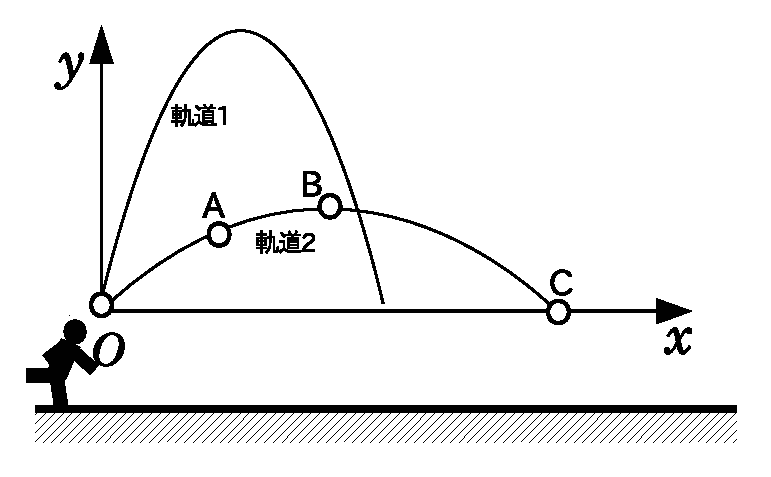
\includegraphics[width=7.0cm]{throwball.eps}
    \caption{ボールの斜め投げ上げ}\label{fig:throwball}
\end{figure}

軌道1のようにかなり上向きに投げ上げたら, 高くは上がるものの, 遠くには飛ばない。軌道2のように, 
若干水平ぎみに投げ上げたら, 高くは上がらないが, そこそこ遠くに飛ぶ。

\begin{q}\label{q:2Dthrow0} 軌道2で, A, B, Cのそれぞれの位置にボールが来た時を考える。
\begin{enumerate}
\item 速さが最も大きいのは, A, B, Cのうちどの位置のときか?
\item A, B, Cの各位置で, ボールにかかる合力を, 矢印で図に描き込め。
矢印の長さは適当でよいが, 複数の矢印どうしで長さはつじつまがあって
いなければならない(大きい力は長く, 小さい力は短く)。
\item A, B, Cの各位置で, ボールの加速度を, 点線矢印で図に描き込め。
矢印の長さは適当でよいが, 複数の矢印どうしで長さはつじつまがあって
いなければならない(大きい加速度は長く, 小さい加速度は短く)。
\item 加速度の大きさが最も大きいのは, A, B, Cのうちどの位置のときか?
\end{enumerate}
\end{q}

\begin{q}\label{q:2Dthrow}
どのような角度で投げ上げたら, 最も遠くまでボールを飛ばせるか, 考えよう。
君の位置を原点$O$とし, 水平方向に$x$軸, 鉛直方向に$y$軸をとる。 時刻を$t$とし, 君がボールを
手放した瞬間を$t=0$とする。$t=0$のときにボールの速度は$x$軸から角$\theta$の方向で, その大きさ
は$v_0$であったとする。

時刻$t$におけるボールの位置と速度をそれぞれ${\bf r}(t), {\bf v}(t)$とする。
重力加速度を$g$とする。
\begin{eqnarray*}{\bf r}(t)=(x(t), y(t))\end{eqnarray*}
とする。
\begin{enumerate}
\item ${\bf r}(0)=(0, 0)$, ${\bf v}(0)=(v_0\cos\theta, v_0\sin\theta)$であることを示せ。
\item ボールが手を離れてから地上に落ちるまでのボールの運動方程式は, 
次式のようになることを示せ:
\begin{eqnarray}
&&m\frac{d^2x}{dt^2}=0\label{eq:2Dthroweqmx}\\
&&m\frac{d^2y}{dt^2}=-mg\label{eq:2Dthroweqmy}
\end{eqnarray}
\item 上の微分方程式(\ref{eq:2Dthroweqmx}), (\ref{eq:2Dthroweqmy})を解くと, 
解はそれぞれ次式のようになることを示せ:
\begin{eqnarray}
&&x=(v_0\cos\theta)t\\
&&y=(v_0\sin\theta)t-\frac{1}{2}\,gt^2
\end{eqnarray}
\item 前問の結果から$t$を消去して次式を示せ:
\begin{eqnarray}
y=(\tan\theta)x-\frac{g}{2v_0^2\cos^2\theta}\,x^2\label{eq:throwtilt}
\end{eqnarray}
\item 前問の結果を, 横軸$x$, 縦軸$y$のグラフに描け。これがボールの軌跡だ。
\item 投げ上げたボールが着地する場所の$x$座標を$X$とすると, 次式を示せ:
\begin{eqnarray}
X=\frac{v_0^2\sin2\theta}{g}\label{eq:throwtiltX}
\end{eqnarray}
\item $v_0$が一定の時, 投げ上げの角$\theta$がどのくらいのとき, $X$は最大になるか? 
\end{enumerate}
\end{q}
\vspace{0.2cm}

\begin{q}\label{q:2Dthrow_hammer}
ハンマー投は, ハンマー(ワイヤーの先に質量7.26~kgの金属球がついたもの)を振り回して投げ上げ, 
飛ばした距離を競うスポーツである。世界記録は86.7~mである。投げ上げの角度が, 前問で求めた角に
一致していたと仮定して, 世界記録樹立時のハンマーの初速度を推定せよ。
\end{q}
\vspace{0.6cm}



\section{円運動}\index{えんうんどう@円運動}

一定の速さで円周上を一方向に動く運動のことを, 等速円運動という。

平面内の円運動を考えてみよう。$xy$座標系の中に質量$m$の質点があり, 何かの機構に
よって, 原点の方向に, 一定の大きさ$F$の力でひっぱられて
いるとしよう(図\ref{fig:circular_motion})。
\begin{figure}[h]
    \centering
    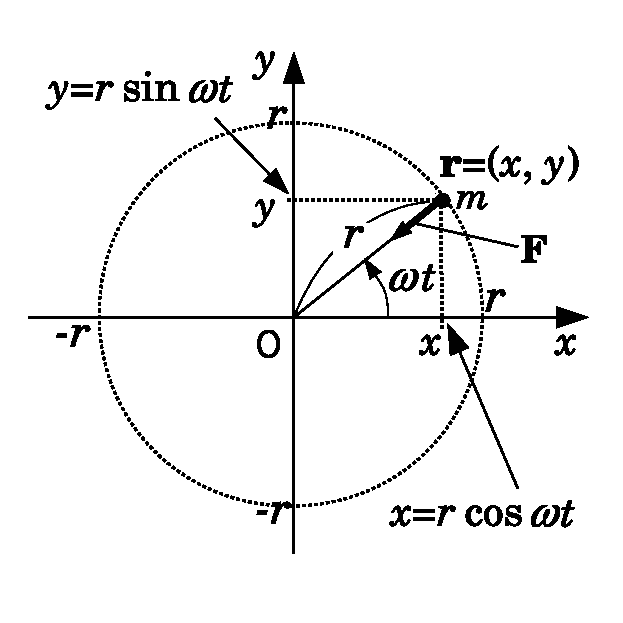
\includegraphics[width=7.0cm]{circular_motion.eps}
    \caption{等速円運動}\label{fig:circular_motion}
\end{figure}
うまく条件が揃えば, この質点は, 原点を中心とする半径$r$の円周上を
等速円運動する。そのことを証明しよう。

まず, 時刻$t$における質点の位置, 速度, 加速度をそれぞれ
\begin{eqnarray}
{\bf r}(t)&=&(x(t), y(t))\\
{\bf v}(t)&=&(v_x(t), v_y(t))\\
{\bf a}(t)&=&(a_x(t), a_y(t))
\end{eqnarray}
とし\footnote{前章でも述べたが, 位置ベクトルは, {\bf r}と書くことも多い。}, 
$t=0$で質点は$x$軸上の点$(r, 0)$にあるとする。すなわち, 
\begin{eqnarray}
{\bf r}(0)=(x(0), y(0))=(r, 0)
\end{eqnarray}
である。

\begin{q}\label{q:circle_motion}
\begin{enumerate}
\item 質点が実際にこの円周上を一定の角速度$\omega$で回転するならば
次式が成り立つことを示せ(ヒント: 極座標):
\begin{eqnarray}
&&{\bf r}(t)=(r\cos\omega t, r\sin\omega t)\label{eq:circle_motion_xy}\\
&&{\bf v}(t)=(-r\omega\sin\omega t, r\omega\cos\omega t)\label{eq:circle_motion_vxvy}\\
&&{\bf a}(t)=(-r\omega^2\cos\omega t, -r\omega^2\sin\omega t)\label{eq:circle_motion_axay}\,\,\,\,\,\,\,\\
&&{\bf a}(t)=-\omega^2{\bf r}(t)\label{eq:circle_motion_a}
\end{eqnarray}
\item 時刻$t$のとき質点に働く力${\bf F}(t)$は, 次式になることを示せ:
\begin{eqnarray}{\bf F}=(-F\cos\omega t, -F\sin\omega t)\end{eqnarray}
\item 質点の運動方程式は, 次式のようになることを示せ:
\begin{eqnarray}
-F\cos\omega t=ma_x(t)\label{eq:circle_motion_Fx}\\
-F\sin\omega t=ma_y(t)\label{eq:circle_motion_Fy}
\end{eqnarray}
\item \eref{eq:circle_motion_axay}で表される$a_x(t), a_y(t)$は, 
次式が成り立つときに限って上の運動方程式を満たす, ということを示せ。
\begin{eqnarray}
F=mr\omega^2\label{eq:mromegasq}
\end{eqnarray}
\item 質点の速度${\bf v}$の大きさ$v$は次式となることを示せ。
\begin{eqnarray}
v=r\omega\label{eq:circle_motion_v_romega}
\end{eqnarray}
\item \eref{eq:mromegasq}は, 次式のようにもできることを示せ:
\begin{eqnarray}
F=\frac{mv^2}{r}\label{eq:mvsqovr}
\end{eqnarray}
\item 質量と半径はそのままで, 速度の大きさ$v$が2倍になると, 力は何倍になるか? 
\item 質量と速度はそのままで, 半径$r$が1/2倍になると, 力は何倍になるか? 
\end{enumerate}
\end{q}
\vspace{0.2cm}

\begin{q}\label{q:car_slip}
前問の最後の結果から, 車を運転する時に, なぜカーブの手前で減速せねばならないか, 述べよ。
\end{q}
\vspace{0.2cm}

%向心力と遠心力



実は, 単振動と円運動は, 密接な関係がある。等速円運動の方程式の
ひとつである\eref{eq:circle_motion_a}を考えよう:
\begin{eqnarray*}
{\bf a}(t)=-\omega^2{\bf r}(t)
\end{eqnarray*}
この左辺は$d^2{\bf r}/dt^2$であり, さらに, ${\bf r}=(x, y)$とおけば, 上の式は, 
\begin{eqnarray}
&&\frac{d^2 x}{dt^2}=-\omega^2 x\\
&&\frac{d^2 y}{dt^2}=-\omega^2 y
\end{eqnarray}
となる。これらは, \eref{eq:vib}と同じ形, すなわち単振動の微分方程式
だ。従って, 等速円運動は, 2つの単振動 ($x$軸方向と$y$軸方向)
の組み合わせと考えることができる。実際, 等速円運動
\begin{eqnarray}\bigl(x(t), y(t)\bigr)=(r\cos\omega t, r\sin\omega t)\end{eqnarray}
について, その$x$座標だけを取り出した関数
\begin{eqnarray}x(t)=r\cos\omega t\end{eqnarray}
は, \eref{eq:spring_Acos}にそっくりだし, $y$座標だけを取り出した関数
\begin{eqnarray}y(t)=r\sin\omega t\end{eqnarray}
は, \eref{eq:spring_Asin}にそっくりだ。
従って, 角速度, 周期などの概念は, 円運動と単振動で共通だ。
ただし, 「角速度」の「角」は, 円運動の場合は幾何学的な意味が
直感的にわかりやすい。
\vspace{0.2cm}

\begin{q}\label{q:hammer_throw}
ハンマー投の世界記録樹立時(問\ref{q:2Dthrow_hammer}参照)に, 投擲者の腕にはどのくらいの力
がかかっただろうか? 
それは何kgの物体を持ち上げる力に相当するだろうか? 回転の半径を1.5~mと仮定せよ(有効数字2桁で十分)。
ヒント:\eref{eq:mvsqovr}。$m$や$v$の値は問\ref{q:2Dthrow_hammer}から流用する。
\end{q}
\vspace{0.2cm}

\begin{q}\label{q:sun_earth0}
太陽のまわりをまわる地球の円運動を考えよう。地球を質点とし, 地球の公転軌道を半径$r$
の円とし(厳密には楕円だが), その中心に太陽があるとし, 太陽は動かないと仮定する。
太陽と地球の質量をそれぞれ$M$, $m$とする。万有引力定数を$G$とする。
\begin{enumerate}
\item この円運動を維持するために地球が太陽から受ける力の大きさを, $r$, $\omega$, $m$であらわせ。
\item この力は万有引力によって実現される。このことから, 次式を示せ。ただし$\omega$は角速度である。
\begin{eqnarray}\omega=\sqrt{\frac{GM}{r^3}}\label{eq:circle_grav_omega}\end{eqnarray}
\item この円運動の周期$T$は, 次式のようになることを示せ:
\begin{eqnarray}T=2\pi\sqrt{\frac{r^3}{GM}}\label{eq:circle_grav_T}\end{eqnarray}
\item $r$, $G$, $M$に具体的な数値を代入して$\omega$の値を求め, 周期を求めよ。それは何日に相当するか? 
(計算に必要な数値は, 各自, 調べよ)
\end{enumerate}
\end{q}
\vspace{0.2cm}

\begin{q}\label{q:spaceship}
以下の宇宙飛行体は, それぞれ何時間で地球のまわりを一周するか? 地球の半径を6400 kmとし, 
地球や以下の飛行体を質点とみなす。()内は地表から飛行体への距離である。
\begin{enumerate}
\item 国際宇宙ステーション(約400 km)
\item 気象衛星ひまわり(約36000 km)
\end{enumerate}
\end{q}

気象衛星ひまわりは, 赤道上空の宇宙空間を, 地球の自転と同じ角速度で地球のまわりを
まわっているので, 常に地表の同じ場所の雲の様子を時々刻々と観測できる。
\mv

\begin{faq}{\small\textgt{自然界には, 円運動だけでなく楕円運動もあるのですか? もしあるなら, やはり運動方程式
で表せるのですか?} ... 
はい。惑星の公転は, 一般には円ではなく楕円であり, やはり運動方程式に従います。特に火星の楕円軌道は, 
「天体は真円運動をする」というオカルト的な中世の思い込みから脱皮してニュートン力学が生まれるための, 
重要な手がかりでした。また, GPS衛星を補完して測量精度を上げるための「みちびき」という日本の
人工衛星(その信号が農地のトラクターの自動運転などで使われている)は, 
気象衛星ひまわりの近くだけど楕円の軌道を動いています。}\end{faq}\mv

\begin{faq}{\small\textgt{公式がごちゃごちゃになってしまいます。。。} ... 
どの式がどの法則から派生するのか, という体系性を意識することが重要。物理学は
公式の羅列ではなく, 法則の体系ですから。}\end{faq}\mv

\begin{faq}{\small\textgt{高校の物理の先生が「物理ができるかどうかは
絵が上手に描けるかどうかで決まる」と言っていました。
確かに絵が上手に描けるとちょっとやる気もでます。。。} ... 
絵や文など, 自分を表現するツールを豊かに持っている人は, 
知的な成長が早いと思います。}\end{faq}\mv

\begin{faq}{\small\textgt{そもそも物の動きとか, わかって何が嬉しいのですか? 
そういうのって, 病気を治す薬とか, バイオ燃料を作る微生物とか, 乾燥に強い植物とかの
研究開発に関係あるのでしょうか?} ... そう短絡的に考えてはダメです。薬の働き方は
タンパク質の構造や, それが酸性度や温度でどう変わるか, などで決まります。それを
知るには, 結局は分子を構成する原子の「動き」が大事なのです。微生物の中の生体反応
も同じ。植物が水を吸い上げるときは, 結局は水分子が「どう動くか」が大事でしょ。
結局, 科学の本質は「動き」に代表される物理現象に帰着するのです。ここで学んでいる
のは, それらの基礎中の基礎です。}\end{faq}\mv

\begin{faq}{\small\textgt{そんなの屁理屈にしか聞こえませんが} ... 
屁理屈ではありませんよ。実際, 薬の分子の動態を, 膨大な数の方程式で表してコンピュータで
解析することが, 既に行われています。そうすることで, 試験管で実験するよりも効率的に, 
たくさんの分子を調べることができるのです。}\end{faq}\mv
\hv

\begin{exq} 
\begin{enumerate}
\item 自転車競技場(競輪場)のトラックのカーブ部分は斜面になっている。その理由を
物理学的に説明せよ。
\item 飛行機(旅客機)に乗ったことのある人は, 飛行機が旋回するとき, 機体を傾ける
ということを知っているだろう。飛行機が左に旋回するとき, 左の翼は上げるか, 下げるか?
その理由を物理学的に説明せよ。(1)とは違う理由であることに注意!
\item 無重力だが空気はある, という環境(国際宇宙ステーションの中など)で紙飛行機を飛ばしたら, どのような運動をするか?
\end{enumerate}
\end{exq}



\section{解答}
%
\noindent{\textbf{答}}\ref{q:harmonic_osci0}
$\omega=\sqrt{k/m}$より, 質量$m$が2倍になると, 角速度$\omega$は$1/\sqrt{2}\fallingdotseq0.71$倍になる
(つまり振動はゆっくりになる)。また, 周期を$T$とすると, $T=2\pi/\omega$だから, $T$は$\sqrt{2}\fallingdotseq1.4$倍になる。\mv

%
\noindent{\textbf{答}}\ref{q:harmonic_osci1}
\eref{eq:lincombvib3}で, $x(0)=X_0$, $x'(0)=0$とすると, $x(t)=X_0\cos\omega t$。
グラフは図\ref{fig:springX0}のようになる。
\begin{figure}[h]
    \centering
    \includegraphics[width=7cm]{springX0.eps}
    \caption{単振動する質点の位置の経時変化}\label{fig:springX0}
\end{figure}

%
\noindent{\textbf{答}}\ref{q:harmonic_osci2}
\eref{eq:lincombvib3}で, $x(0)=0$, $x'(0)=V_0$とすると, 
\begin{eqnarray}x(t)=\frac{V_0}{\omega}\sin\omega t\end{eqnarray}
となる。グラフは図\ref{fig:springV0}のようになる。\mv
\begin{figure}[h]
    \centering
    \includegraphics[width=7cm]{springV0.eps}
    \caption{単振動する質点の速度の経時変化}\label{fig:springV0}
\end{figure}

% 君は地表のある点から, 空にむかって, 斜め方向に質量
\noindent{\textbf{答}}\ref{q:2Dthrow0} 略。ヒント: 飛行中のボールに
働く力は重力のみ(空気抵抗は無視している)。\\

\noindent{\textbf{答}}\ref{q:2Dthrow}
${\bf r}(t)=(x(t), y(t))$, ${\bf v}(t)=(x'(t), y'(t))$となることに注意せよ。
\begin{enumerate}
\item ボールは時刻$t=0$で原点(君の位置)にあるから${\bf r}(0)=(0,0)$。
また, $|{\bf v}(0)|=v_0$で, ${\bf v}(0)$が$x$軸からなす角が$\theta$であること
から, 
\begin{eqnarray}{\bf v}(0)=(v_0\cos\theta, v_0\sin\theta)\end{eqnarray}
\item $x$方向には力が働かないので, \eref{eq:2Dthroweqmx}が成り立つ。
$y$方向には重力つまり$-mg$が働くので, \eref{eq:2Dthroweqmy}が成り立つ。
\item \eref{eq:2Dthroweqmx}を2回積分すると, 
\begin{eqnarray}x(t)=C_1t+C_2\end{eqnarray}
となる。ここで$C_1, C_2$は積分定数。
$x(0)=0$より$C_2=0$。$x'(0)=v_0\cos\theta$より, $C_1=v_0\cos\theta$。
従って, 
\begin{eqnarray}x(t)=(v_0\cos\theta)t\end{eqnarray}
\eref{eq:2Dthroweqmy}を2回積分すると, 
\begin{eqnarray}y(t)=-\frac{gt^2}{2}+C_3t+C_4\end{eqnarray}
となる。ここで$C_3, C_4$は積分定数。
$y(0)=0$より$C_4=0$。$y'(0)=v_0\sin\theta$より, $C_3=v_0\sin\theta$。
従って, 
\begin{eqnarray}y(t)=(v_0\sin\theta)t-\frac{gt^2}{2}\end{eqnarray}
\item 略(各自計算せよ)。
\item 図\ref{fig:throw_ball_slant}
\begin{figure}[h]
    \centering
    \includegraphics[width=8cm]{throw_ball_slant.eps}
    \caption{斜めに投げ上げられたボールの軌跡}\label{fig:throw_ball_slant}
\end{figure}
\item 略(\eref{eq:throwtilt}で$y=0$となるのは, $x=0$と\eref{eq:throwtiltX}
の場合であり, 前者は投げ上げの瞬間, 
後者は着地の瞬間に対応する。$2\cos\theta\sin\theta=\sin2\theta$に注意せよ。)
\item \eref{eq:throwtiltX}が最大になるのは, $\theta=\pi/4$, つまり45度のとき。
\end{enumerate}
\mv

\noindent{\textbf{答}}\ref{q:2Dthrow_hammer}
前問より, $\theta=\pi/4$が, ハンマー投擲の最適角度。このとき\eref{eq:throwtiltX}
は$X=v_0^2/g$となる。従って$v_0=\sqrt{gX}$。$X=86.7$~m, 
$g=9.8$~m~s$^{-2}$とすれば, $v_0=29.1$~m~s$^{-1}$。
\mv

% 平面内の円運動を考えてみよう
\noindent{\textbf{答}}\ref{q:circle_motion}
\begin{enumerate}
\item 略(数学リメディアル教材参照)
\item 原点から質点へのベクトル(つまり質点の位置ベクトル)は
\begin{eqnarray}
{\bf r}&=&(r\cos\omega t, r\sin\omega t)\nonumber\\
       &=&r(\cos\omega t, \sin\omega t)
\end{eqnarray}
だから, 原点から質点へ向かう単位ベクトルは$(\cos\omega t, \sin\omega t)$。問題の仮定より, 
質点にかかる力の方向は, 質点から原点への方向である。その方向の単位ベクトルは, 前述の単位ベクトル
の逆向きだから, $(-\cos\omega t, -\sin\omega t)$。力の大きさは$F$なので, 結局, 力を
あらわすベクトルは, 以下のようになる:
\begin{eqnarray}
{\bf F}(t)&=&F(-\cos\omega t, -\sin\omega t)\nonumber\\
          &=&(-F\cos\omega t, -F\sin\omega t)
\end{eqnarray}
\item 略($x, y$各方向の運動方程式を考えればよい)。
\item \eref{eq:circle_motion_axay}で表された$a_x(t), a_y(t)$を\eref{eq:circle_motion_Fx}, \eref{eq:circle_motion_Fy}に代入すれば, 
\begin{eqnarray}
-F\cos\omega t=-mr\omega^2\cos\omega t\\
-F\sin\omega t=-mr\omega^2\sin\omega t
\end{eqnarray}
となる。前者の両辺を$-\cos\omega t$で割ったり, 後者の両辺を$-\sin\omega t$で割ったり
すれば, $F=mr\omega^2$, すなわち\eref{eq:mromegasq}が成り立つ。逆に, \eref{eq:mromegasq}
が成り立てば, 上記の式が成り立つのは明らかだ。
\item 略(\eref{eq:circle_motion_vxvy}を使って$(v_x, v_y)$の大きさを求めるだけ)。
\item 略(\eref{eq:circle_motion_v_romega}と\eref{eq:mromegasq}から$\omega$を消去)。
\item \eref{eq:mvsqovr}より, 4倍。
\item \eref{eq:mvsqovr}より, 2倍。
\end{enumerate}
\mv

%
\noindent{\textbf{答}}\ref{q:car_slip}
タイヤは高速で転がっていても, 地面との接触面は常に地面と噛み合って
いるので, 接触面ではタイヤと地面は静止しているため, 摩擦力は静止摩擦力である。

さて, 車がカーブに入ると, その回転運動を維持するには, 前問の結果から, 
速度の二乗に比例した横向きの力を, 車のタイヤと地面の間での摩擦力で実現しなければ
ならない。従って, 高速度でカーブに入ると, 激しく大きな静止摩擦力が要求される。
それに耐えきれないと, タイヤと地面の間で滑りが起き, 突然, 摩擦力は静止摩擦力
から, より小さな動摩擦力に代わるので, 車はカーブを続けることができなくなる。
カーブに入ってから慌てて急ブレーキを踏むと, さらに大変なことになる。
ブレーキによってタイヤの回転が急に止まるので, 地面とタイヤの間での滑りが, 
より早い段階(車が減速する前)で起きてしまう。そのような事態になっては遅い。
それを避けるには, カーブへ進入する前に十分に減速する必要がある。万一, 
高速度でカーブに入ってしまったら, タイヤがスリップしないように気をつけて
ブレーキをじんわり踏みながら, 幸運を祈るしかない。
\mv

%
\noindent{\textbf{答}}\ref{q:hammer_throw}
投擲者がハンマーを手放す直前まで, ハンマーは回転運動している。その速度を
$v$とすると, \eref{eq:mvsqovr}より, $F=mv^2/r$の力が投擲者の腕にかかった
はずである。問\ref{q:2Dthrow_hammer}の問題文と結果より, $m=7.26$~kg, $v=29.1$~m~s$^{-1}$。$r=1.5$~mとすると, 
$F=4100$ N。これに相当する重力を受ける物体の質量は, この値を$g=9.8$~m~s$^{-2}$で
割って, 約420~kg。つまり約420~kgの物体を地上で持ち上げるのに必要な力に相当する。
\mv

%
\noindent{\textbf{答}}\ref{q:sun_earth0}
\begin{enumerate}
\item \eref{eq:mromegasq}より, $mr\omega^2$
\item 万有引力は$GMm/r^2$。従って, 
\begin{eqnarray}mr\omega^2=\frac{GMm}{r^2}\end{eqnarray}
これを$\omega$について解けば与式を得る。
\item $T=2\pi/\omega$より与式を得る。
\item $G=6.67408\times10^{-11}$ N~m$^2$~kg$^{-2}$, $M=1.9891\times10^{30}$~kg, 
$r=1.4960\times10^{11}$~mとすると, $\omega=1.99125\times10^{-7}$ Hz。
周期は, $2\pi/\omega=3.15539\times10^7$~s$=365.207$~日=$365.21$~日。
注: 実際の公転周期365.25~日と少しずれたのは, 地球は厳密には楕円軌道をしているため。
これを補正するには$r$の値に修正が必要。
注: 与えられた数値は有効数字5桁であっても, 途中計算は1桁余分にとって行い, 最後に5桁に丸める。
\end{enumerate}
\mv

%
\noindent{\textbf{答}}\ref{q:spaceship}
\eref{eq:circle_grav_T}において$M$を地球の質量とすればよい。
\begin{enumerate}
\item $r=6800$ kmとすると, $T=5580$ s$\fallingdotseq$1.6時間。
\item $r=42000$ kmとすると, $T=87000$ s$\fallingdotseq$24時間。
\end{enumerate}

